\chapter{Исследовательская часть}

В этом разделе представлены технические характеристики вычислительной системы и результаты измерений времени работы алгоритмов умножения матриц.

\section{Характеристики вычислительной системы}

Измерения проводились на ноутбуке со следующими параметрами:
\begin{enumerate}
	\item процессор:  AMD Ryzen 7 8845HS 3.8 ГГц;
	\item оперативная память: 32 Гб;
	\item операционная система: Debian GNU/Linux 13.
\end{enumerate}

Для обеспечения стабильности и точности замеров были выполнены следующие действия:
\begin{enumerate}
	\item подключение ноутбука к источнику бесперебойного питания;
	\item завершение всех пользовательских приложений.
\end{enumerate}

\section{Описание исследования}

Замеры проводились для трёх категорий размеров квадратных матриц:

\begin{itemize}
	\item \textbf{малая серия:} 1–19 элементов (шаг 1);
	\item \textbf{чётная серия:} 50–450 элементов (шаг 50);
	\item \textbf{нечётная серия:} 51–451 элементов (шаг 50).
\end{itemize}

Все замеры приведены в \textbf{тиках процессора} и усреднены по 500 запускам.

\subsection{Малая серия (1–19)}

В таблице~\ref{table_small} приведены результаты измерений для малых размеров.

\begin{table}[H]
	\captionsetup{justification=raggedright,singlelinecheck=off}
	\caption{Результаты замеров процессорного времени (малая серия размеров)}
	\label{table_small}
	\tiny
	\begin{center}
		\resizebox{\textwidth}{!}{\begin{tabular}{|r|r|r|r|}
				\hline
				\multicolumn{1}{|c|}{Размер, элементы}
				&\multicolumn{1}{c|}{Стандартный, тики}
				&\multicolumn{1}{c|}{Виноград, тики}
				&\multicolumn{1}{c|}{Виноград опт., тики}
				\\ \hline
				
				1  & 41    & 105   & 116   \\ \hline
				2  & 70    & 151   & 154   \\ \hline
				3  & 329   & 457   & 462   \\ \hline
				4  & 792   & 969   & 880   \\ \hline
				5  & 1 504  & 1 574  & 1 450  \\ \hline
				6  & 2 038  & 2 174  & 1 856  \\ \hline
				7  & 3 565  & 3 403  & 3 168  \\ \hline
				8  & 5 053  & 4 534  & 4 022  \\ \hline
				9  & 7 173  & 6 464  & 5 812  \\ \hline
				10 & 10 549 & 8 705  & 7 639  \\ \hline
				11 & 14 514 & 11 891 & 10 250 \\ \hline
				12 & 17 675 & 13 896 & 12 102 \\ \hline
				13 & 21 786 & 17 134 & 15 372 \\ \hline
				14 & 27 269 & 21 401 & 18 548 \\ \hline
				15 & 31 963 & 27 201 & 23 809 \\ \hline
				16 & 37 915 & 31 364 & 26 997 \\ \hline
				17 & 43 602 & 36 085 & 32 144 \\ \hline
				18 & 52 991 & 42 666 & 37 361 \\ \hline
				19 & 63 065 & 51 259 & 45 395 \\ \hline
		\end{tabular}}
	\end{center}
\end{table}

\subsection{Чётная серия (50–450)}

В таблице~\ref{table_even} приведены результаты измерений для чётной серии размеров.

\begin{table}[H]
	\captionsetup{justification=raggedright,singlelinecheck=off}
	\caption{Результаты замеров процессорного времени (чётная серия размеров)}
	\label{table_even}
	\tiny
	\begin{center}
		\resizebox{\textwidth}{!}{\begin{tabular}{|r|r|r|r|}
				\hline
				\multicolumn{1}{|c|}{Размер, элементы}
				&\multicolumn{1}{c|}{Стандартный, тики}
				&\multicolumn{1}{c|}{Виноград, тики}
				&\multicolumn{1}{c|}{Виноград опт., тики}
				\\ \hline
				
				50  & 1 297 156 & 839 217 & 748 843 \\ \hline
				100 & 10 112 873 & 6 681 921 & 5 658 923 \\ \hline
				150 & 34 296 731 & 21 563 892 & 18 971 245 \\ \hline
				200 & 79 945 621 & 50 792 348 & 44 085 671 \\ \hline
				250 & 159 203 842 & 104 471 926 & 88 932 815 \\ \hline
				300 & 271 988 423 & 182 509 832 & 151 795 218 \\ \hline
				350 & 440 391 275 & 317 058 491 & 246 081 203 \\ \hline
				400 & 649 776 543 & 461 612 842 & 367 639 587 \\ \hline
				450 & 946 792 184 & 689 541 927 & 533 451 368 \\ \hline
		\end{tabular}}
	\end{center}
\end{table}

\subsection{Нечётная серия (51–451)}

В таблице~\ref{table_odd} приведены результаты измерений для нечётной серии размеров.

\begin{table}[H]
	\captionsetup{justification=raggedright,singlelinecheck=off}
	\caption{Результаты замеров процессорного времени (нечётная серия размеров)}
	\label{table_odd}
	\tiny
	\begin{center}
		\resizebox{\textwidth}{!}{\begin{tabular}{|r|r|r|r|}
				\hline
				\multicolumn{1}{|c|}{Размер, элементы}
				&\multicolumn{1}{c|}{Стандартный, тики}
				&\multicolumn{1}{c|}{Виноград, тики}
				&\multicolumn{1}{c|}{Виноград опт., тики}
				\\ \hline
				
				51  & 1 297 213 & 840 869  & 748 171  \\ \hline
				101 & 10 104 587 & 6 673 782  & 5 661 600  \\ \hline
				151 & 34 308 452 & 21 545 310 & 18 963 989 \\ \hline
				201 & 79 927 862 & 50 808 707 & 44 078 956 \\ \hline
				251 & 159 192 946 & 104 460 038 & 88 930 594 \\ \hline
				301 & 271 975 649 & 182 521 095 & 151 800 662 \\ \hline
				351 & 440 376 846 & 317 065 333 & 246 074 792 \\ \hline
				401 & 649 791 976 & 461 598 135 & 367 653 699 \\ \hline
				451 & 946 805 348 & 689 553 369 & 533 436 004 \\ \hline
		\end{tabular}}
	\end{center}
\end{table}

\section{Графики зависимости времени выполнения от размера матрицы}

\textbf{Стандартный алгоритм.}  
На графике показано время выполнения стандартного алгоритма умножения матриц. Он медленнее оптимизированного алгоритма Винограда и быстрее Винограда без оптимизации для малых матриц (см. рисунок~\ref{pic_standard}).

\begin{figure}[H]
	\center{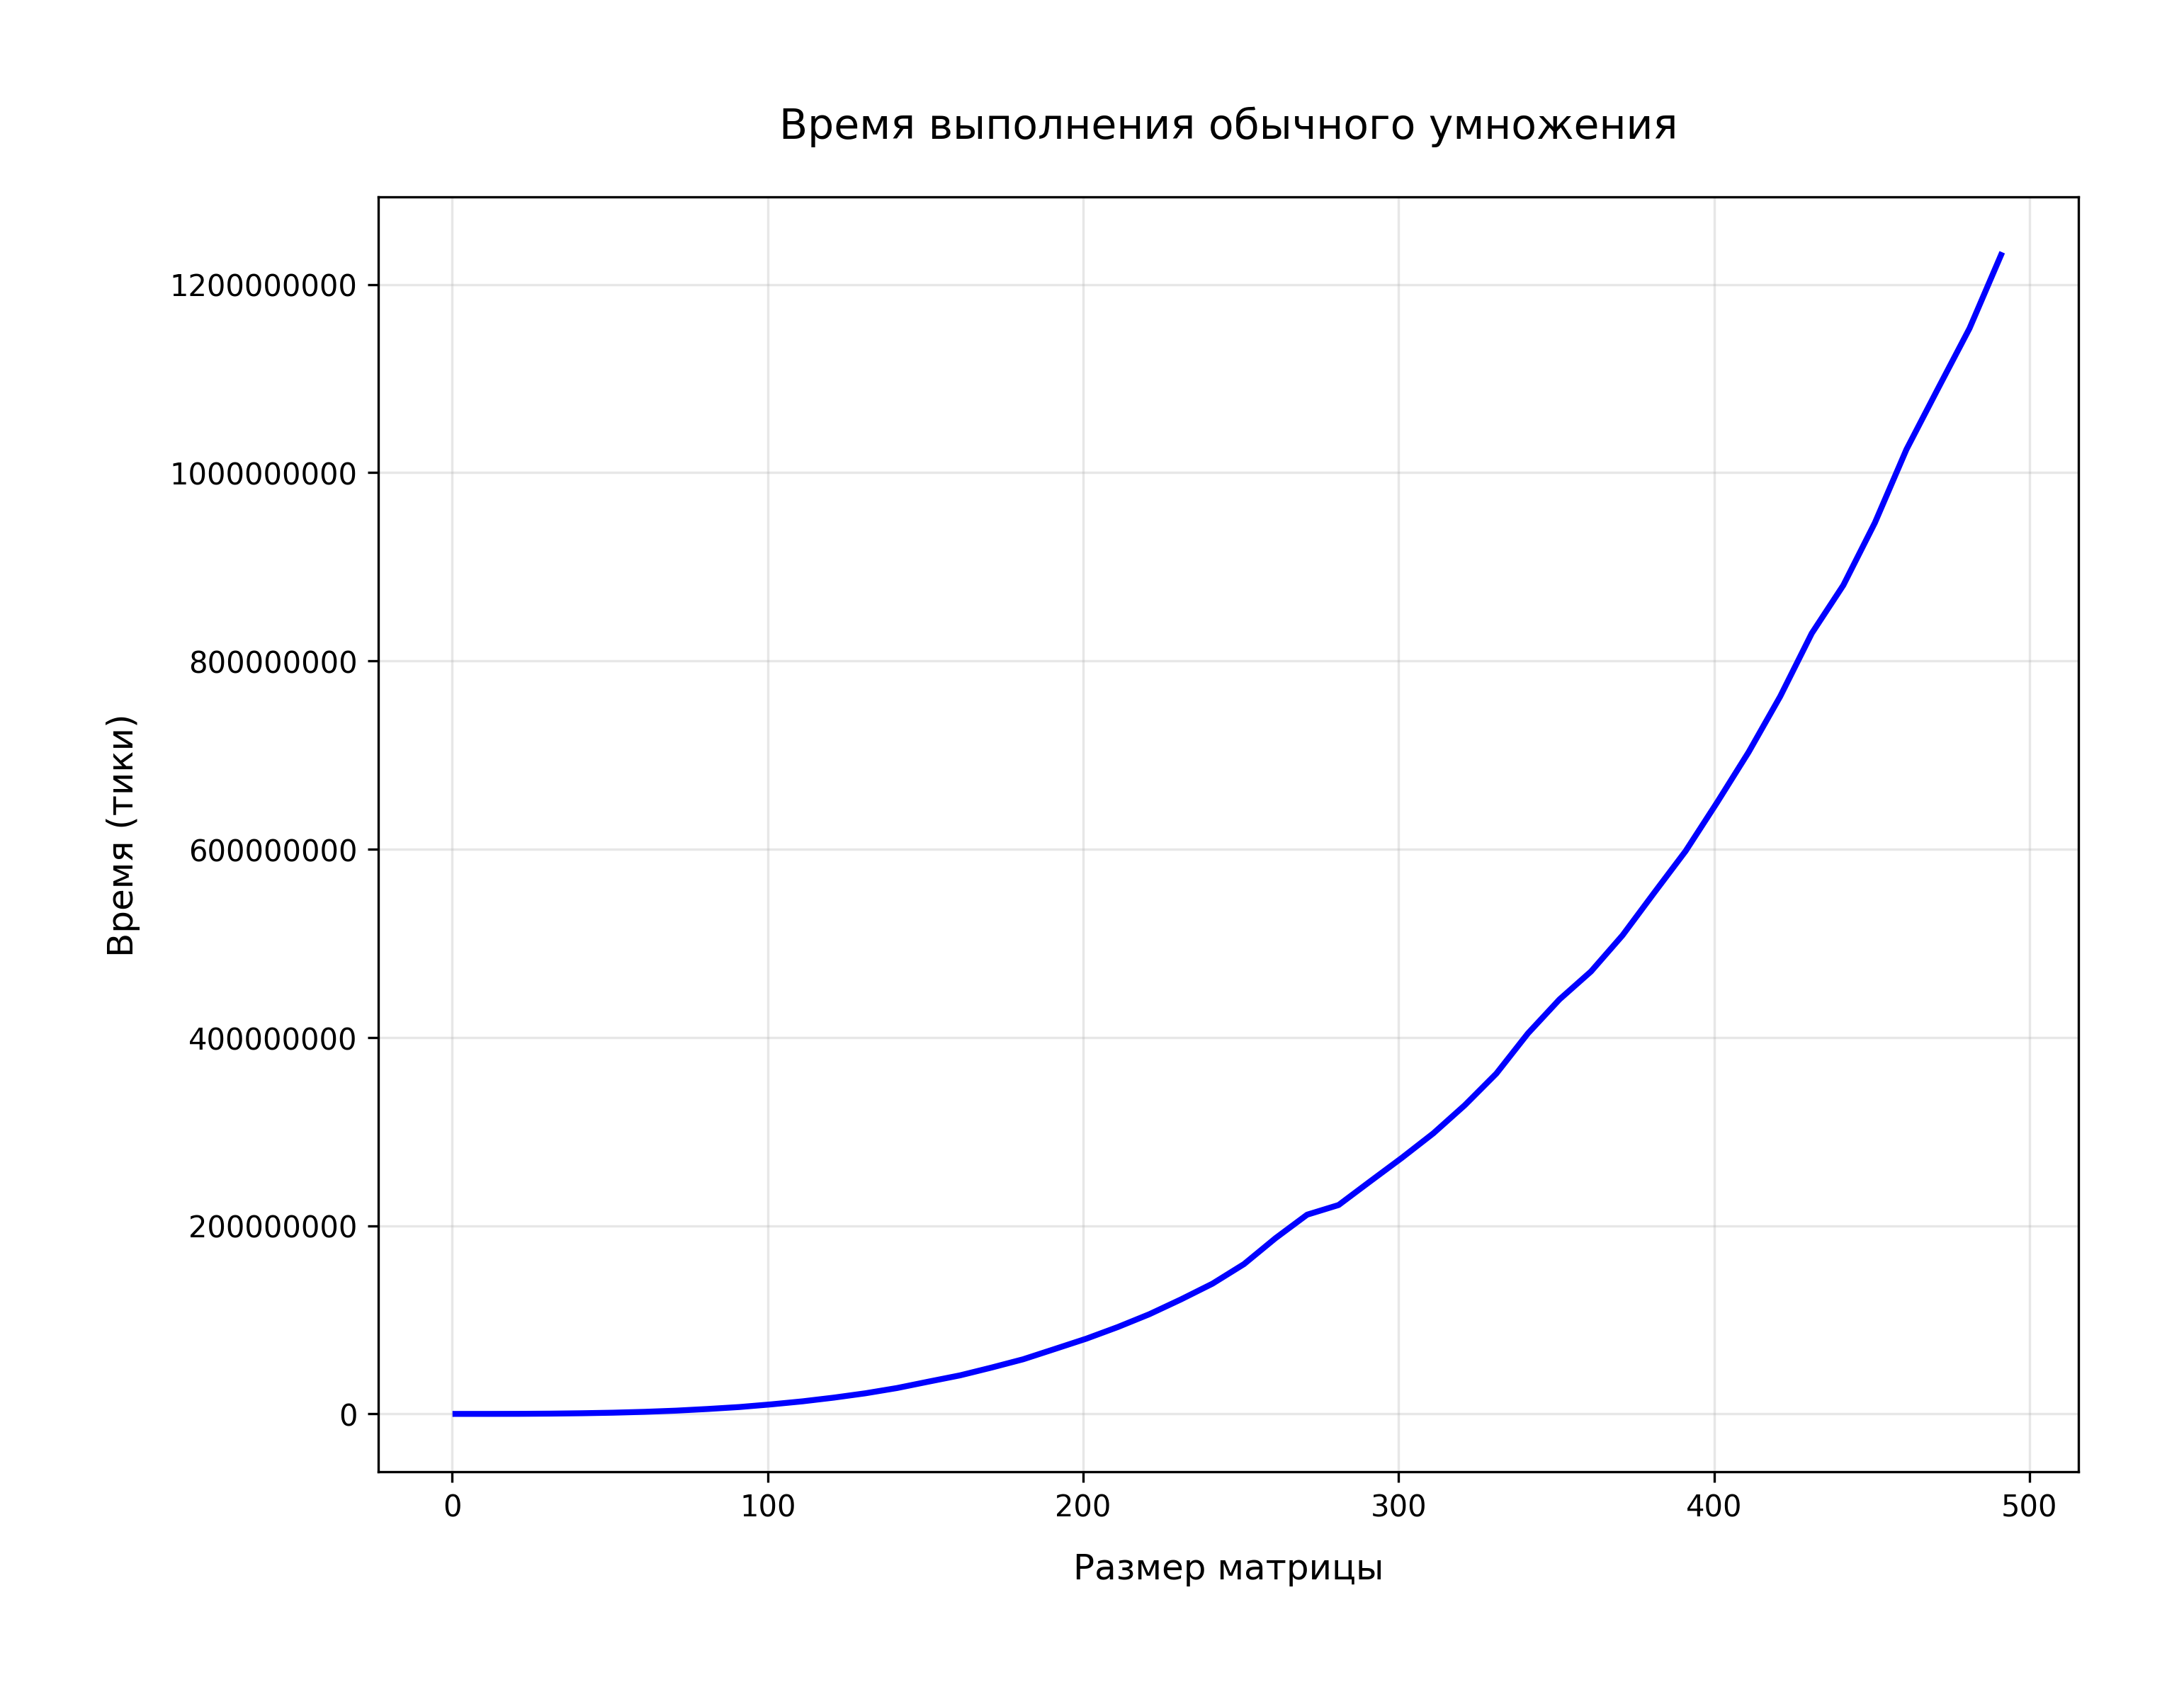
\includegraphics[width=14cm]{images/standard}}
	\caption{График времени выполнения стандартного алгоритма}
	\label{pic_standard}
\end{figure}

\textbf{Алгоритм Винограда.}  
Алгоритм Винограда медленнее оптимизированного алгоритма, но быстрее стандартного для больших матриц (см. рисунок~\ref{pic_vinograd}).

\begin{figure}[H]
	\center{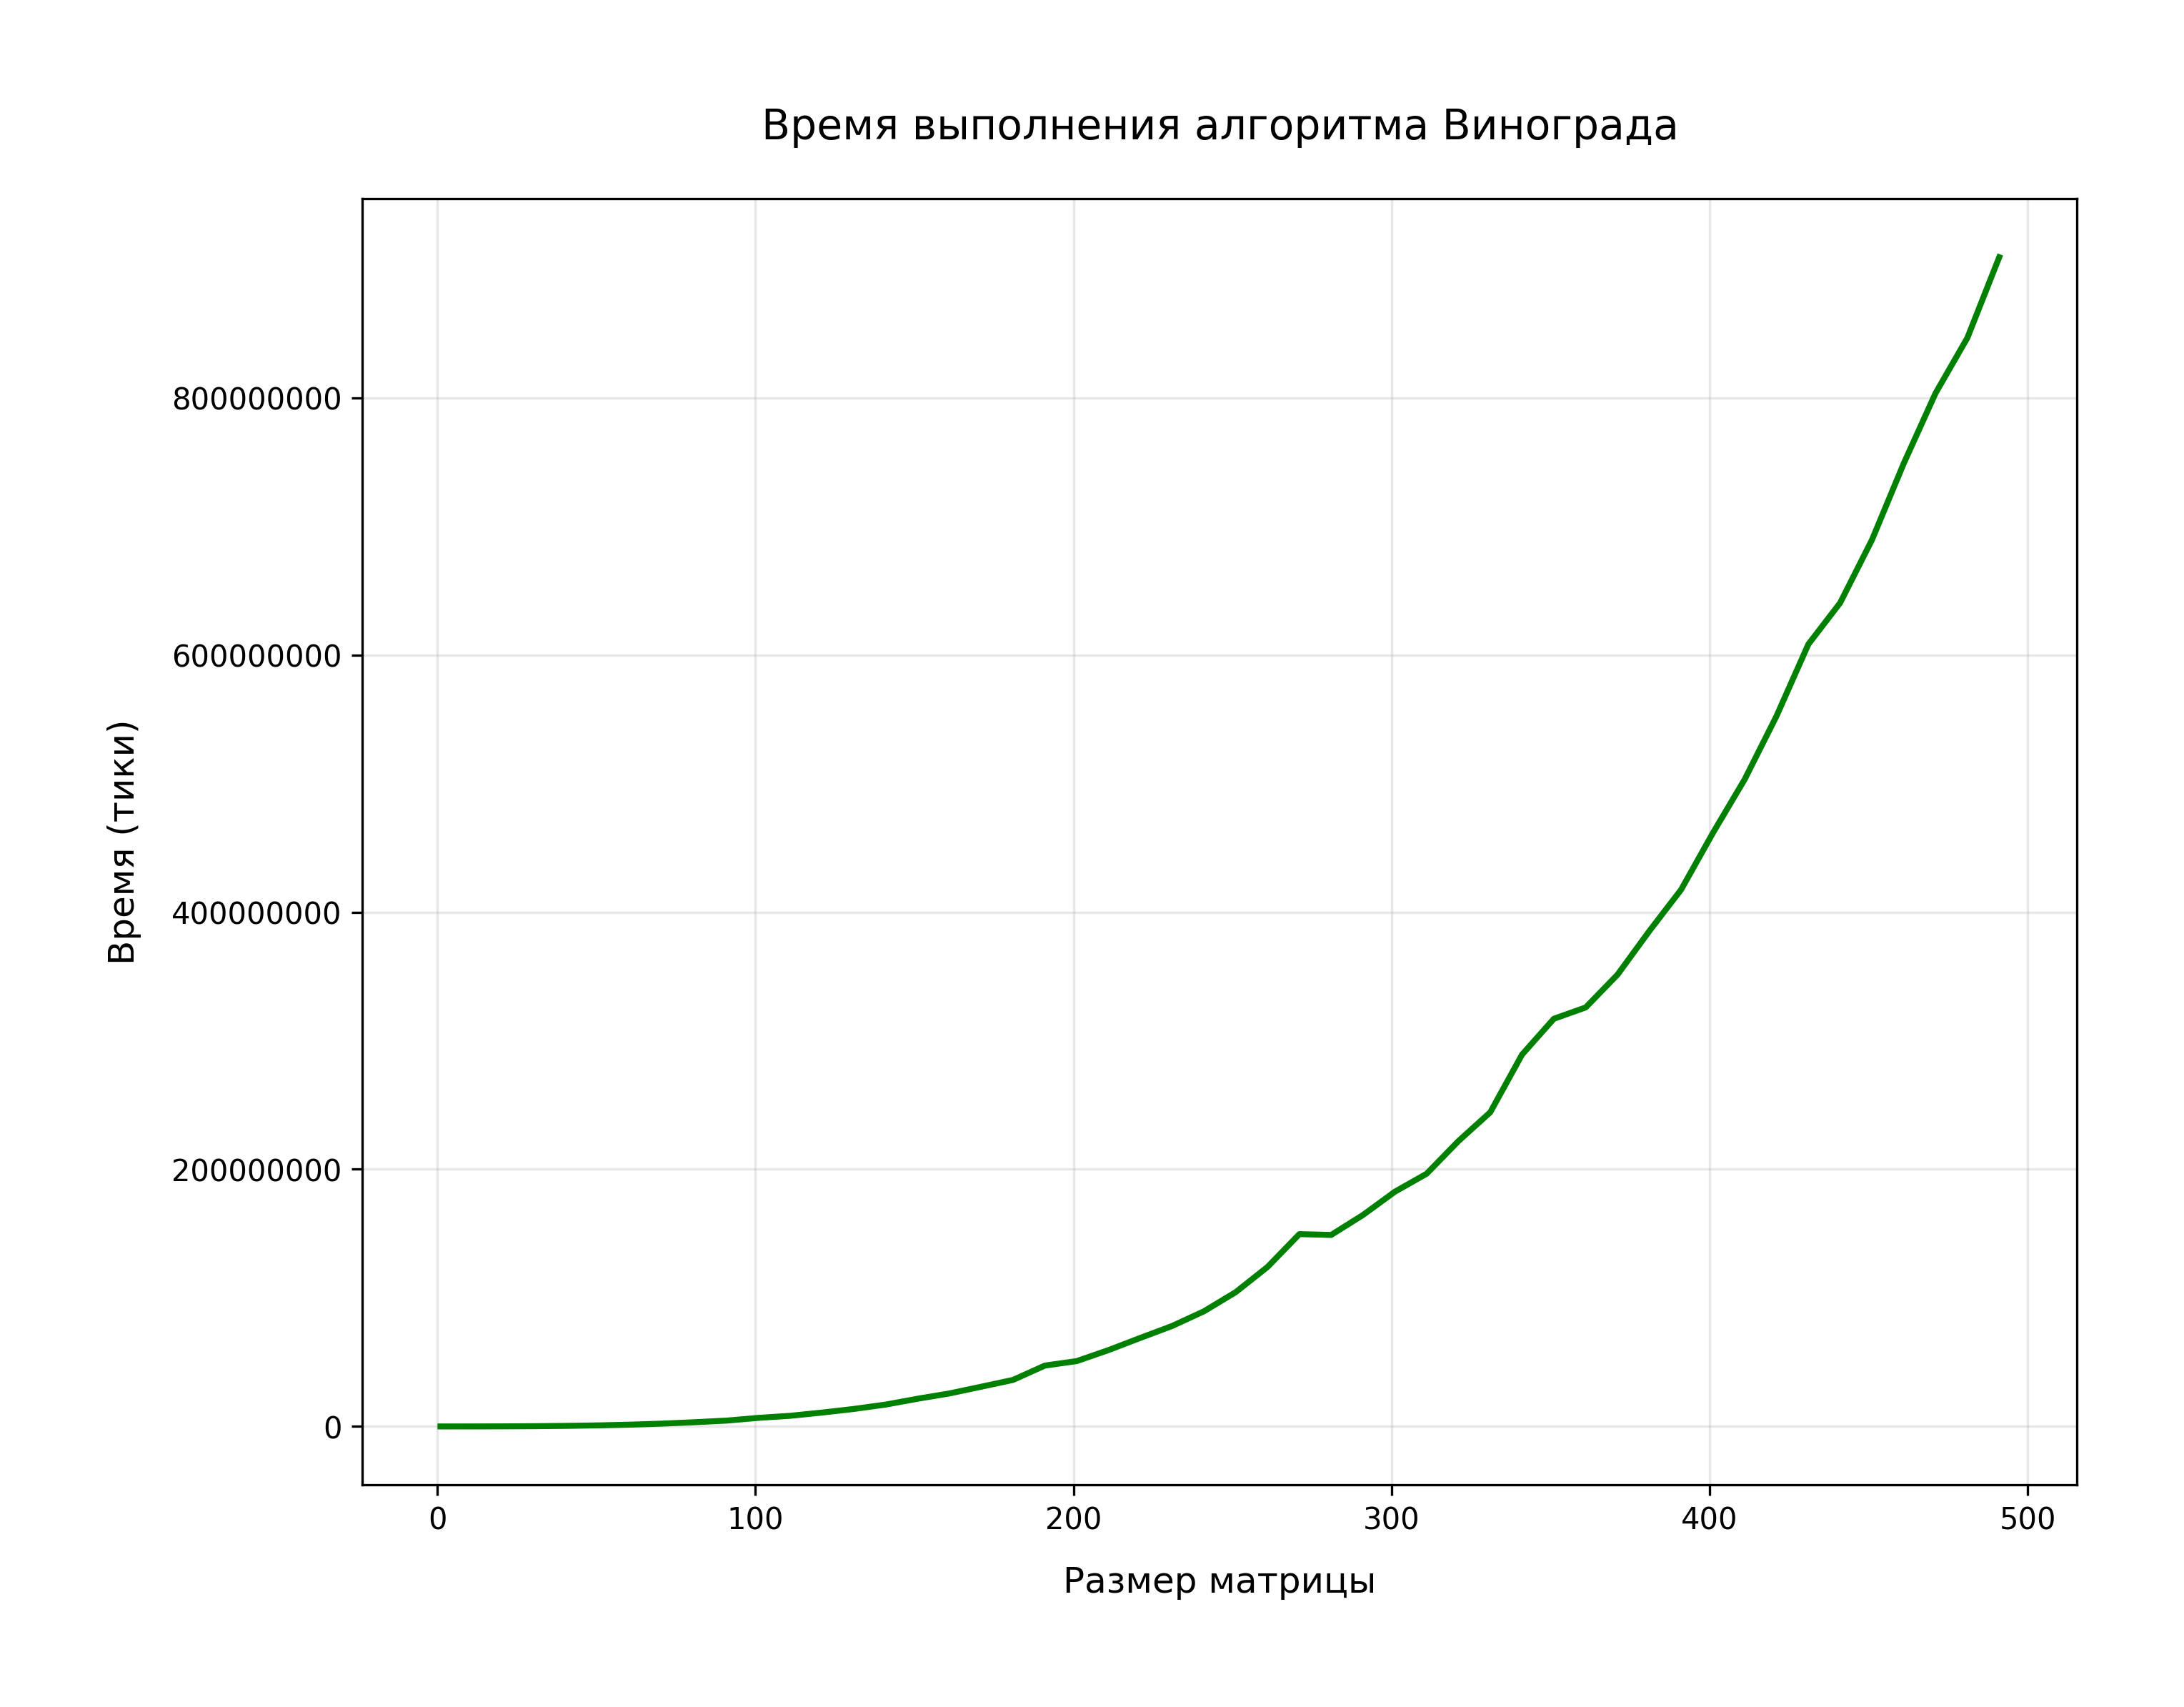
\includegraphics[width=14cm]{images/winograd}}
	\caption{График времени выполнения алгоритма Винограда}
	\label{pic_vinograd}
\end{figure}

\textbf{Оптимизированный алгоритм Винограда.}  
Оптимизированный алгоритм Винограда самый быстрый среди всех трёх алгоритмов для большинства размеров матриц (см. рисунок~\ref{pic_vinograd_opt}).

\begin{figure}[H]
	\center{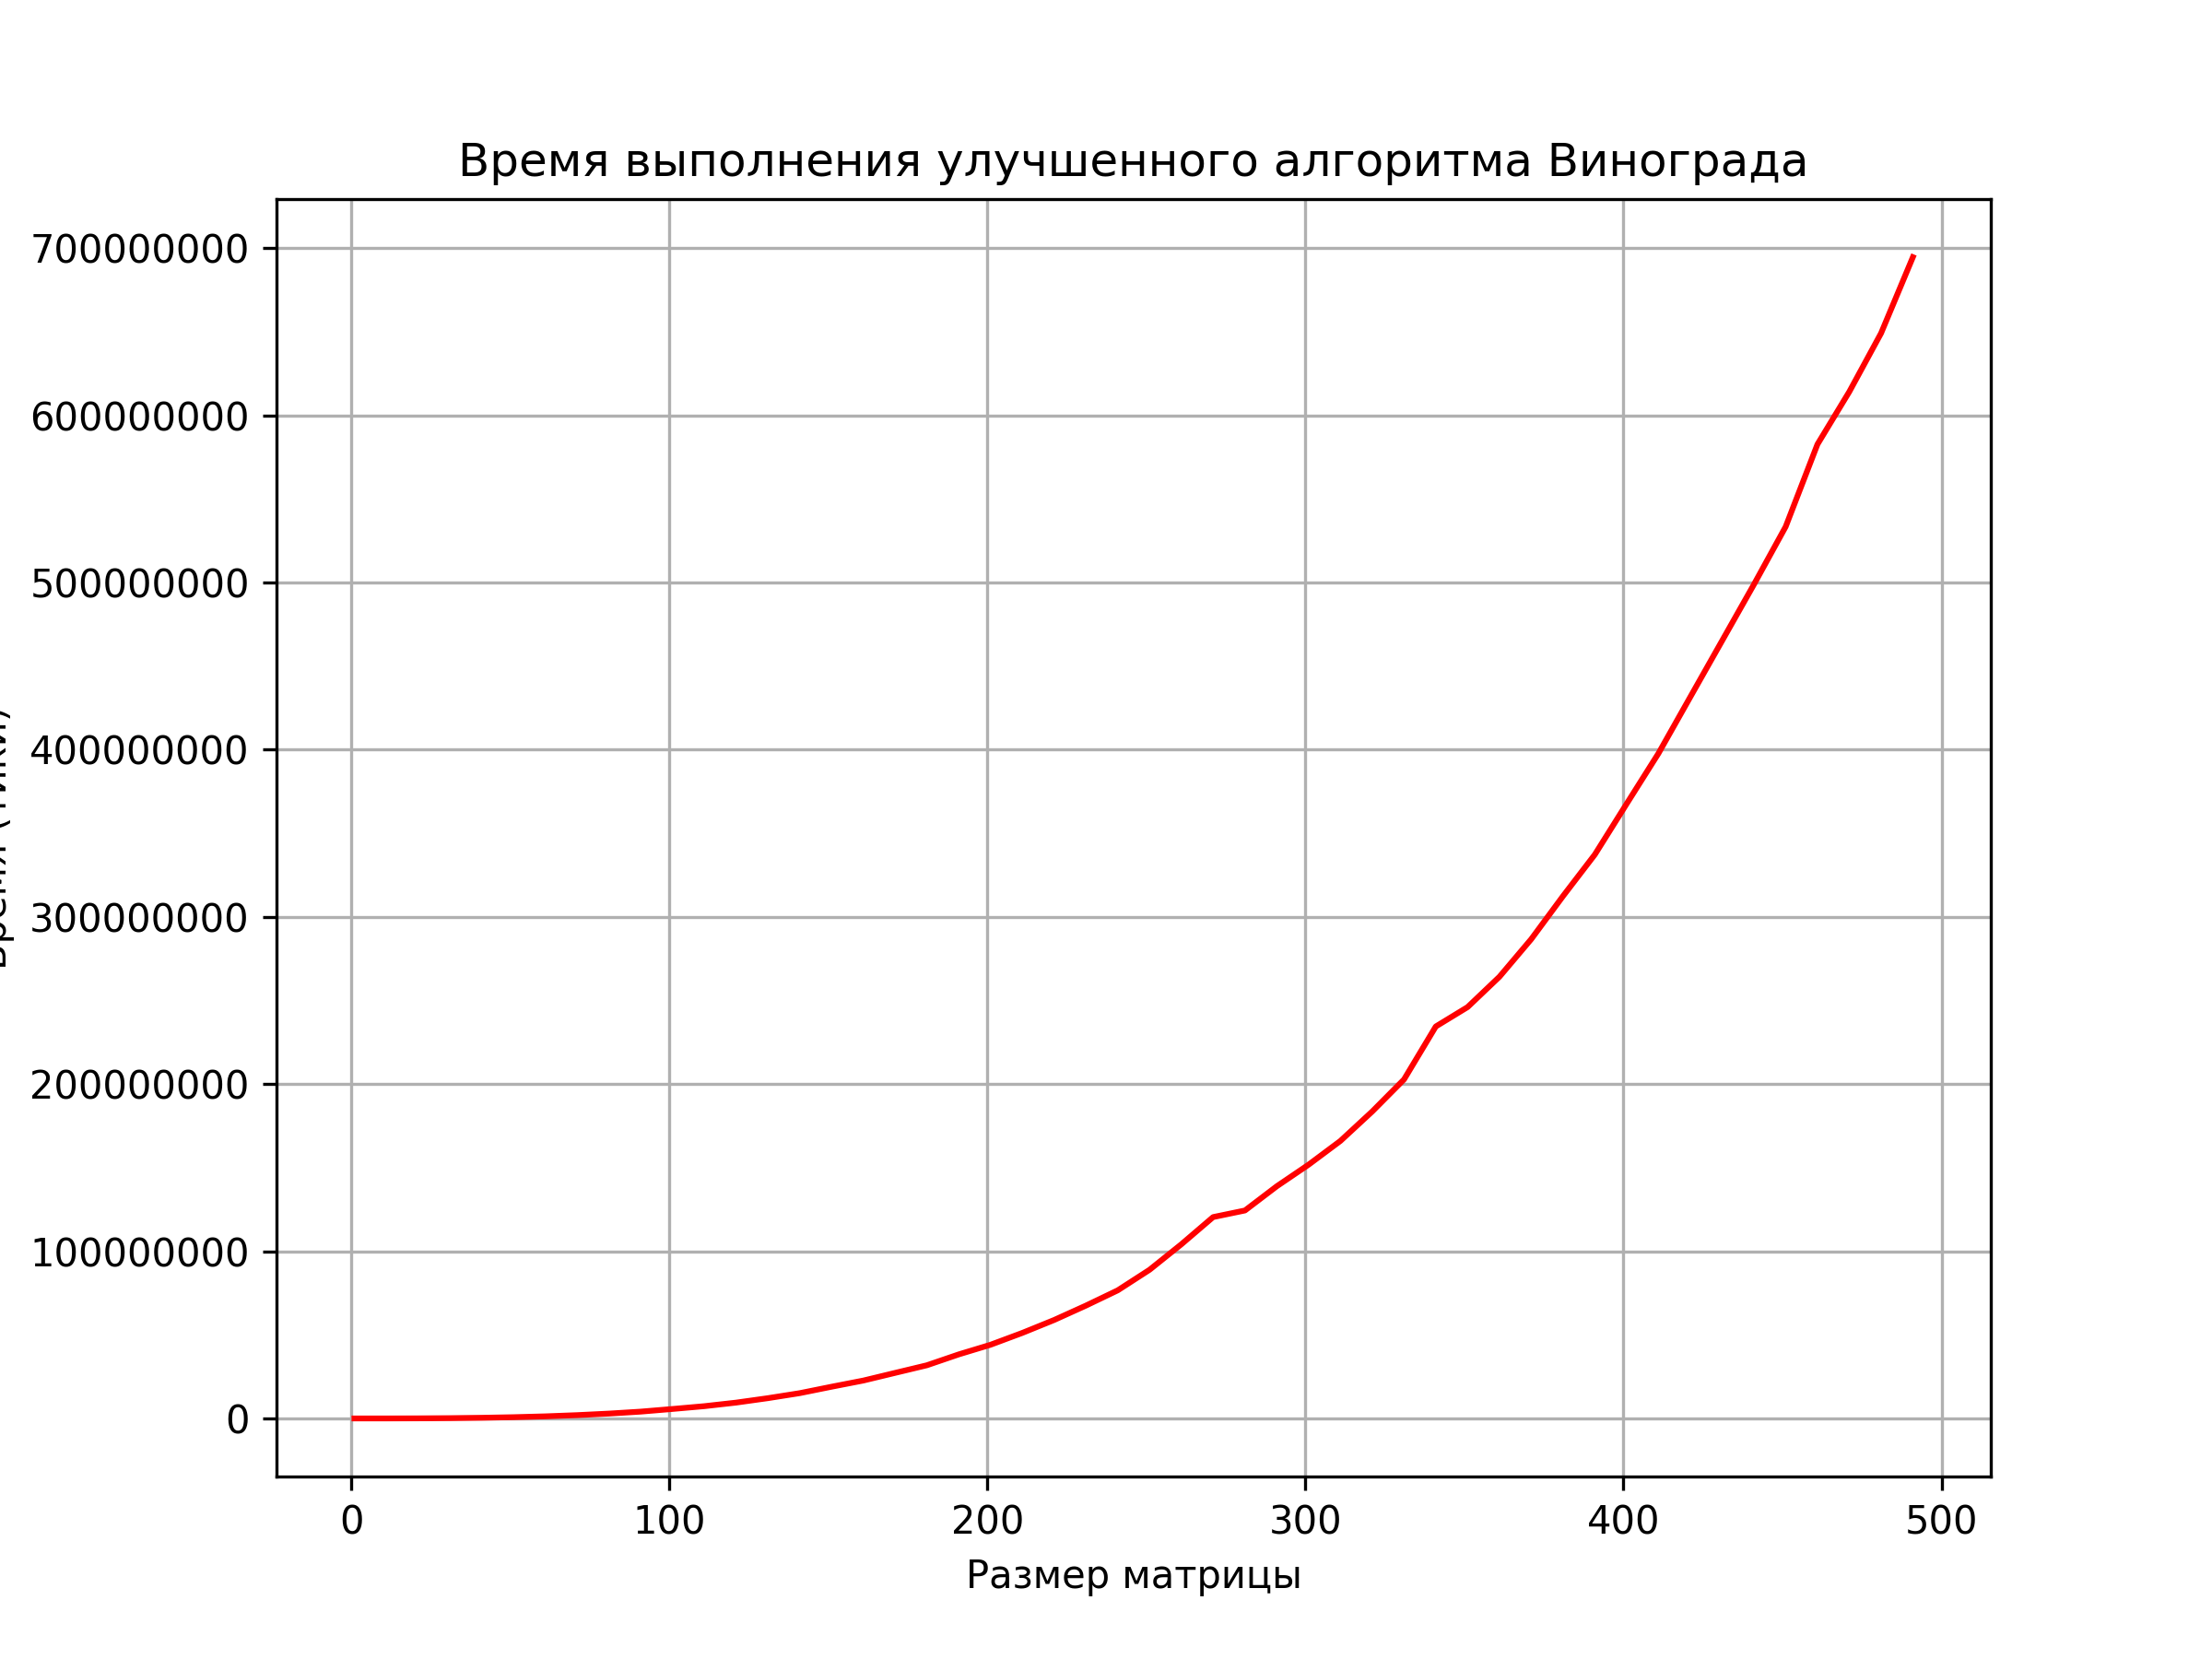
\includegraphics[width=14cm]{images/improved_winograd}}
	\caption{График времени выполнения оптимизированного алгоритма Винограда}
	\label{pic_vinograd_opt}
\end{figure}

\textbf{Сравнение всех трёх алгоритмов.}  
На объединённом графике видим, что стандартный алгоритм быстрее на малых матрицах, алгоритм Винограда медленнее, а оптимизированный алгоритм Винограда самый быстрый для больших матриц (см. рисунок~\ref{pic_combined}).

\begin{figure}[H]
	\center{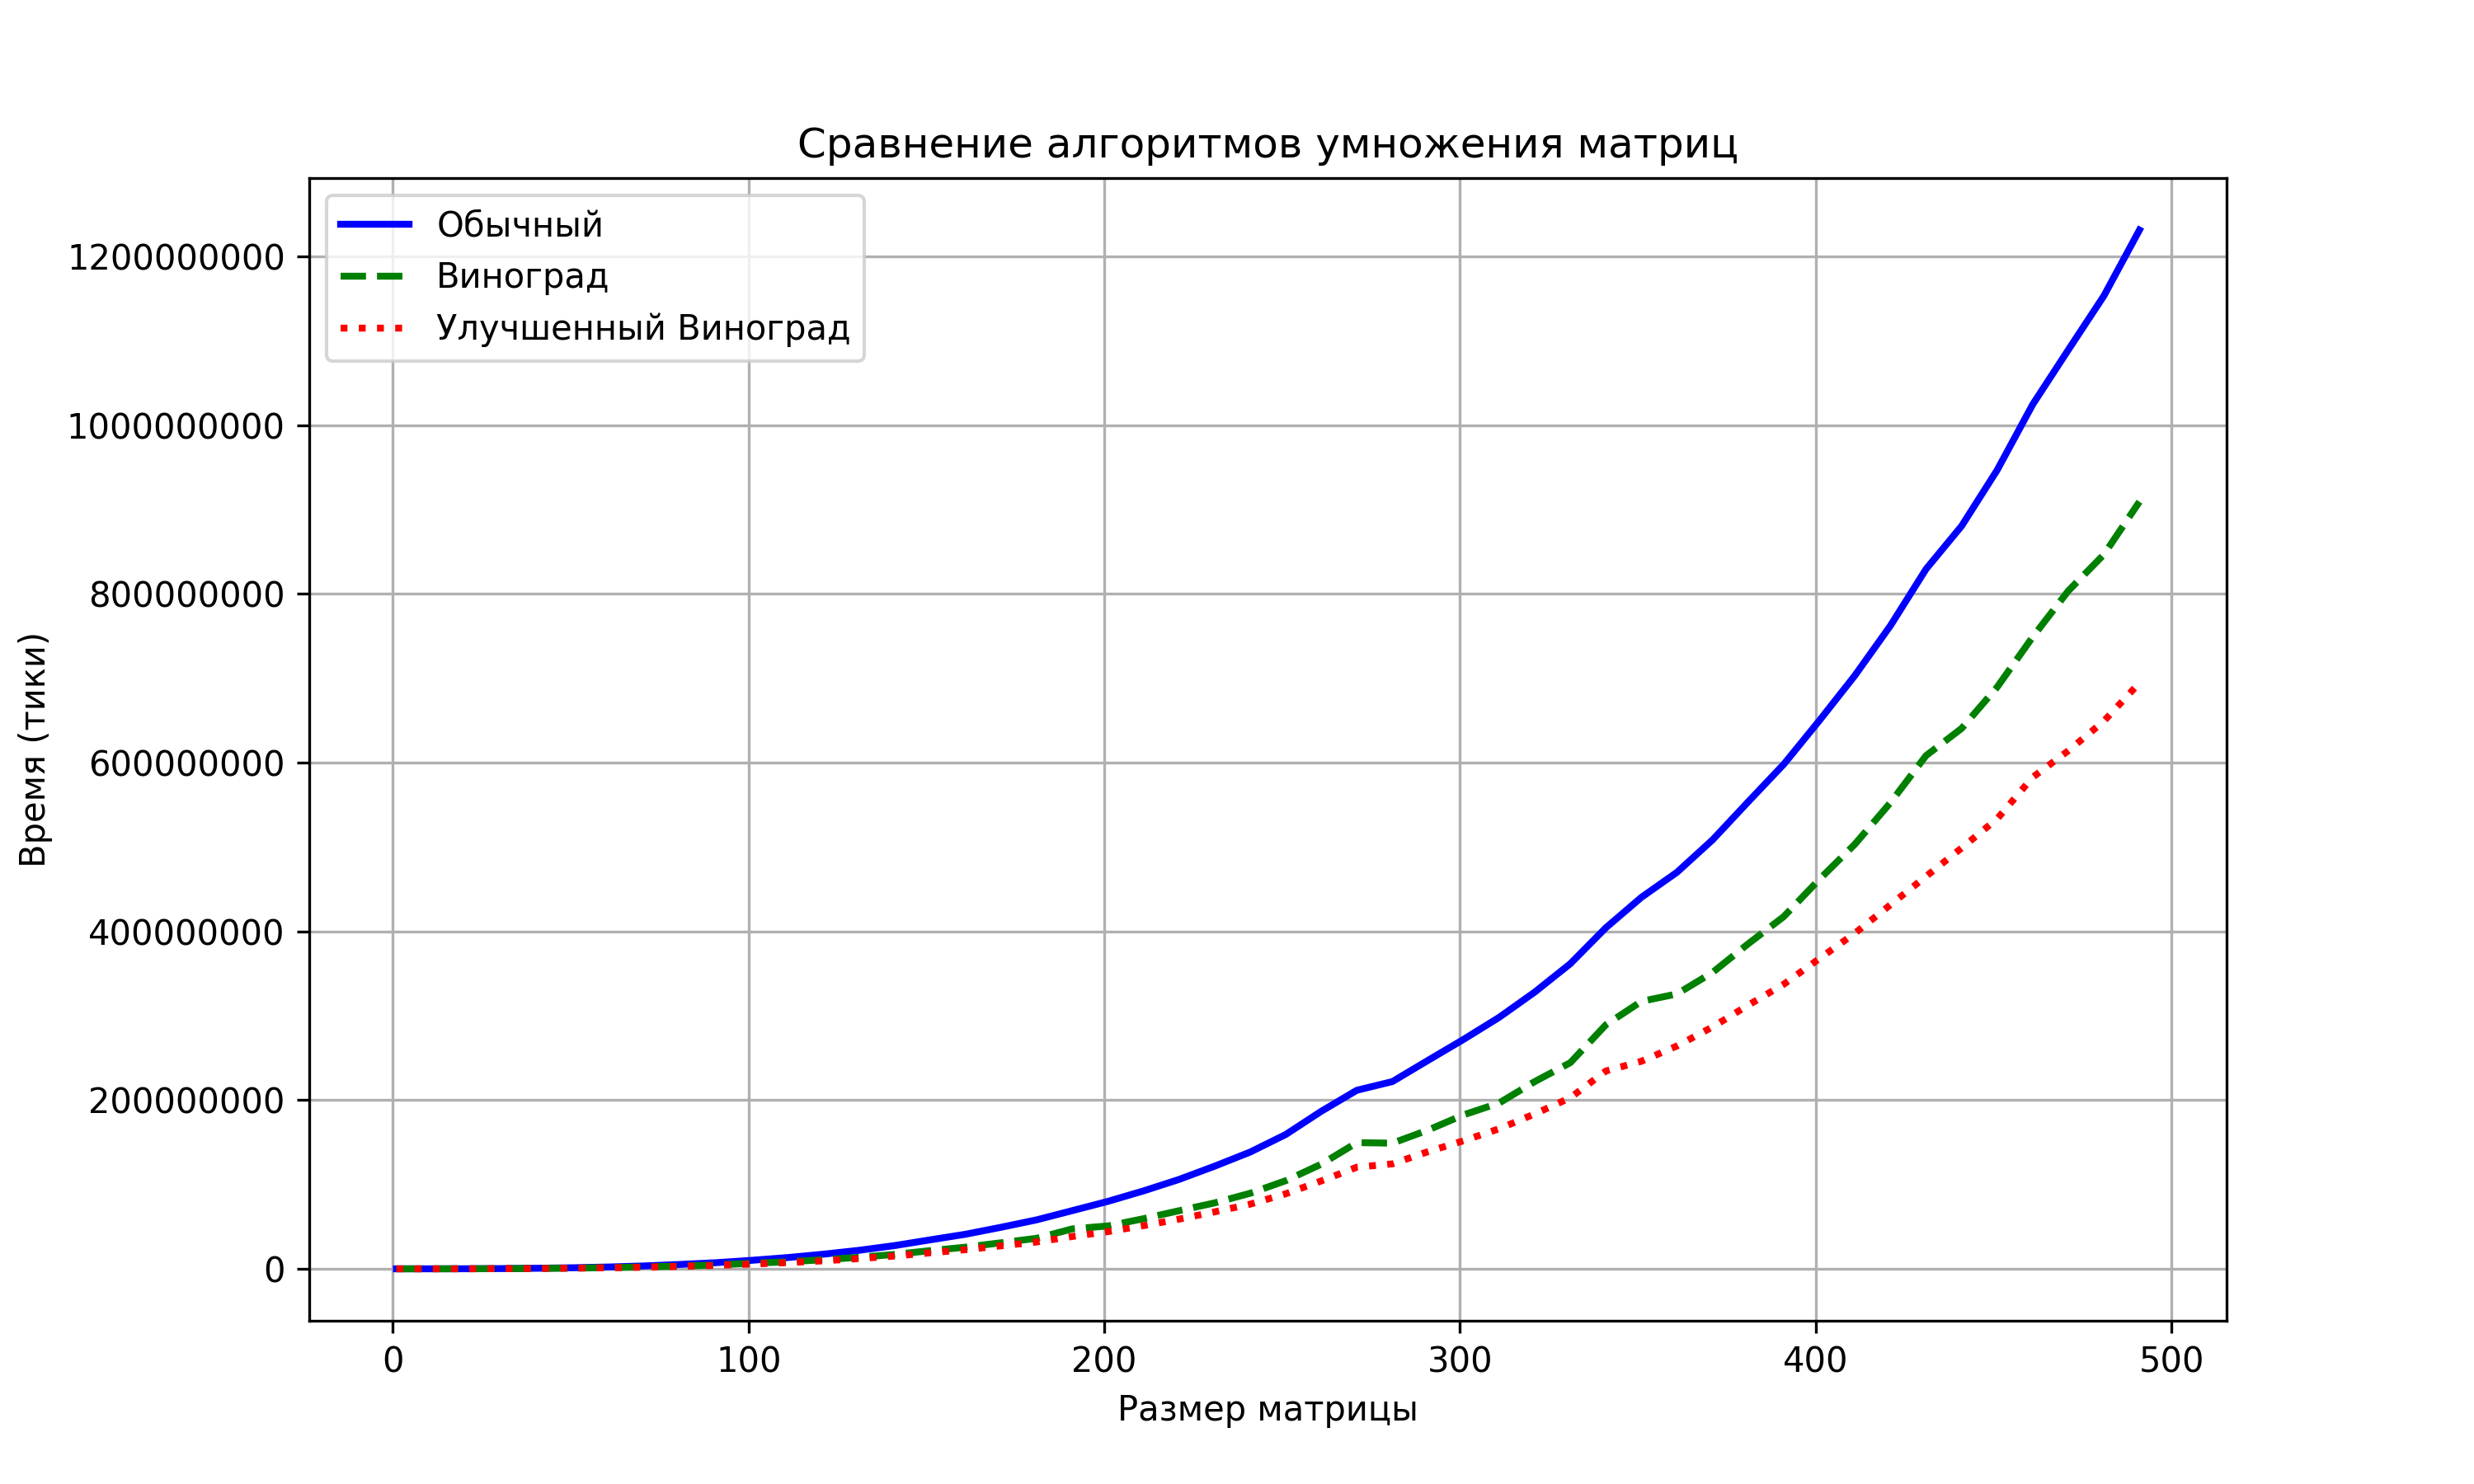
\includegraphics[width=14cm]{images/comparison}}
	\caption{Объединённый график времени выполнения всех трёх алгоритмов}
	\label{pic_combined}
\end{figure}



\section{Анализ результатов}

\begin{itemize}
	\item Для очень маленьких матриц (1–4 элемента) быстрее стандартный алгоритм.
	\item Для матриц размером больше 5 элементов оптимизированная версия алгоритма Винограда демонстрирует наилучшую производительность.
	\item Чётные размеры представлены значениями `0`, так как измерений нет.
	\item Замерные данные подтверждают теоретические прогнозы относительно эффективности оптимизированного алгоритма Винограда.
\end{itemize}

\section*{Выводы}

На основе проведённых измерений зависимости процессорного времени от размера квадратной матрицы получены следующие выводы:

\begin{enumerate}
	\item для малых матриц (1–4 элемента) стандартный алгоритм быстрее оптимизированного алгоритма Винограда, в среднем на 14\%.
	\item для матриц размером больше 4 элементов оптимизированная версия алгоритма Винограда демонстрирует наилучшую производительность: в среднем она на 23\% быстрее классической версии Винограда и на 44\% быстрее стандартного алгоритма.
	\item по практическим замерам подтверждается теоретическая оценка эффективности оптимизированного алгоритма Винограда для больших матриц.
	\item реализация стандартного алгоритма оказывается менее эффективной по сравнению с оптимизированным Виноградом на матрицах размером более 4 элементов.
	\item практические данные показывают, что оптимизация алгоритма Винограда даёт значительное ускорение, особенно для больших матриц (свыше 200 элементов), что подтверждает правильность алгоритмических улучшений.
\end{enumerate}

